\documentclass[10pt]{article}
\usepackage[margin=1in]{geometry}
\usepackage{times}
\usepackage{microtype}
\usepackage{graphicx}
\usepackage{booktabs}
\usepackage{amsmath}
\usepackage{amssymb}

\usepackage{hyperref}
\usepackage{caption}
\usepackage{subcaption}

\hypersetup{
  colorlinks=true,
  linkcolor=blue,
  urlcolor=blue,
  citecolor=blue
}

\newcommand{\AuthorName}{Walid Albasha}
\newcommand{\GithubURL}{https://github.com/albashawalid05-netizen}

\title{\textbf{Neural ODEs vs ResNets under Irregular Sampling (Toy Study)}}
\author{\AuthorName \\
\small \href{\GithubURL}{\GithubURL}}
\date{}

\begin{document}
\maketitle

\begin{abstract}
We compare discrete-time residual networks (ResNets) with continuous-time Neural Ordinary Differential Equations (Neural ODEs) on a synthetic damped oscillator dataset with irregular observation times and controlled missingness. Using a shared training/evaluation pipeline in PyTorch (baselines, metrics, ablations, and plots), we find Neural ODEs substantially outperform a ResNet baseline across all tested conditions. Solver choice (RK4 vs.\ DOPRI5) has negligible effect in this setup, while increasing missingness impacts the ResNet more than the Neural ODE. We discuss likely failure modes, error characteristics, and limitations of this toy study.
\end{abstract}

\vspace{-0.5em}
\section{Problem}
Many sequence models assume regularly sampled observations. In real settings (medical records, sensor networks, event logs), sampling is often \emph{irregular} and observations are \emph{missing}. This project studies a minimal controlled setting: a synthetic damped oscillator with irregular sampling and a missingness mask. We ask:
\begin{quote}
\emph{Under irregular sampling and missingness, do continuous-time Neural ODEs provide an advantage over discrete-time ResNet-style dynamics?}
\end{quote}

\section{Method}
\subsection{Data: Damped oscillator with missingness}
We generate trajectories from a damped oscillator and sample them at irregular time points. Missingness is applied by a mask with a configurable missing rate. The model receives observed values and the missingness pattern and is trained to predict the target trajectory under the same protocol across runs.

\subsection{Models}
\textbf{ResNet baseline.} We implement a step-wise residual network (ResNetStep) that updates hidden state using discrete transitions. Discrete models can struggle when time gaps vary unless time-delta conditioning or continuous interpolation is handled carefully.

\textbf{Neural ODE.} We model hidden dynamics as a continuous-time ODE and solve between observation times using an ODE solver. This provides an inductive bias aligned with irregular sampling: the model naturally handles variable time gaps by integrating over the actual intervals.

\subsection{Training and evaluation}
All experiments share the same training loop and evaluation script. We report mean squared error (MSE) on held-out evaluation data. Each run is driven by a YAML config and logged to JSON; evaluation aggregates into a summary CSV and produces figures.

\section{Experiments}
\subsection{Environment and reproducibility}
\begin{itemize}
  \item OS: Windows; GPU: RTX 4070 Laptop
  \item PyTorch: \texttt{torch 2.7.1+cu118} (\texttt{cuda=True})
  \item Entry points:
  \begin{itemize}
    \item \texttt{python -m src.train --config .\textbackslash configs\textbackslash base.yaml}
    \item \texttt{python -m src.eval}
    \item \texttt{python -m src.plots}
  \end{itemize}
\end{itemize}

\subsection{Runs}
We use the following runs from \texttt{results/tables/summary.csv}:
\begin{itemize}
  \item \textbf{base:} missing=0.3, solver=RK4
  \item \textbf{ablation\_solver\_dopri5:} missing=0.3, solver=DOPRI5
  \item \textbf{ablation\_missing\_0:} missing=0.0
  \item \textbf{ablation\_missing\_60:} missing=0.6
\end{itemize}

\section{Results}
Table~\ref{tab:summary} summarizes MSE across configurations. Neural ODE achieves an order-of-magnitude lower MSE than the ResNet baseline in all runs.

\begin{table}[h]
\centering
\caption{Summary of results (lower MSE is better).}
\label{tab:summary}
\begin{tabular}{lcc}
\toprule
Run (config) & ResNet MSE & Neural ODE MSE \\
\midrule
base (missing=0.3, RK4) & 0.111581 & 0.011062 \\
solver: DOPRI5 & 0.111581 & 0.011063 \\
missing=0.0 & 0.145135 & 0.011394 \\
missing=0.6 & 0.109933 & 0.010556 \\
\bottomrule
\end{tabular}
\end{table}

\subsection{Figures}
\begin{figure}[h]
\centering
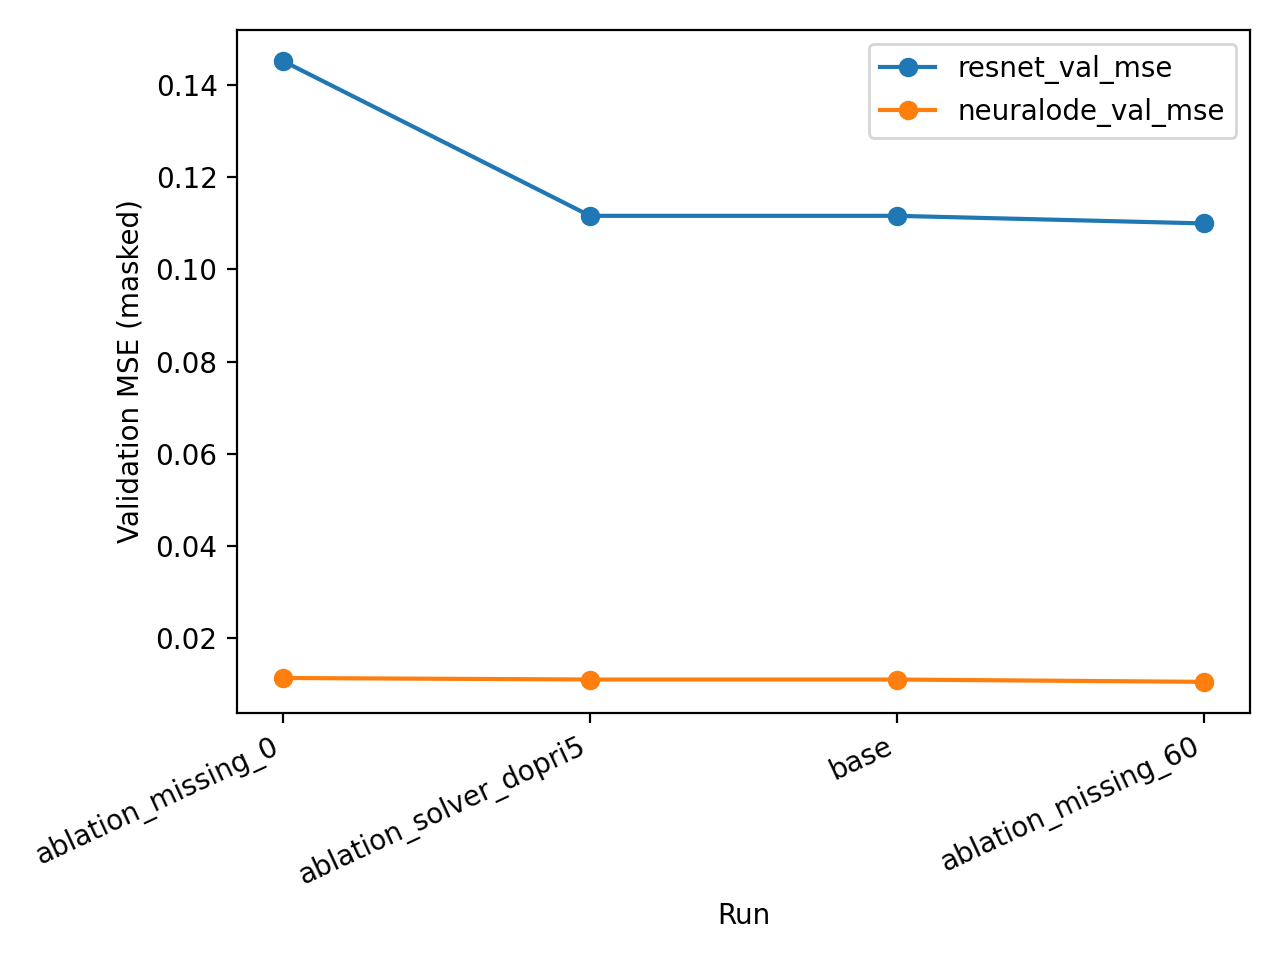
\includegraphics[width=0.95\linewidth]{../results/figures/mse_by_run.png}
\caption{MSE by run/config. Neural ODE is consistently lower.}
\label{fig:mse_by_run}
\end{figure}

\begin{figure}[h]
\centering
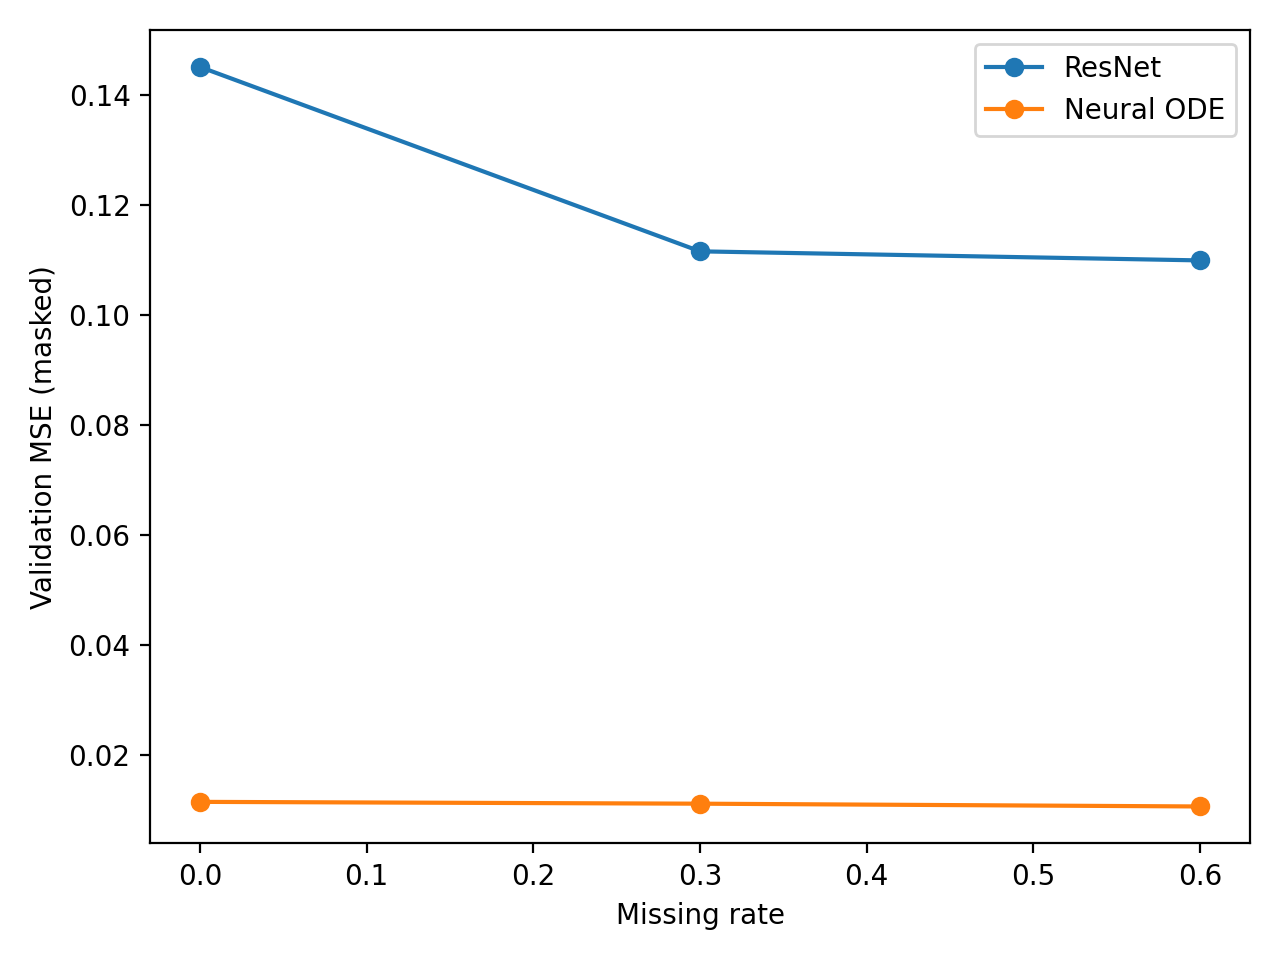
\includegraphics[width=0.95\linewidth]{../results/figures/mse_vs_missing_rate.png}
\caption{MSE vs missing rate. Neural ODE remains stable; ResNet varies more.}
\label{fig:mse_vs_missing}
\end{figure}

\section{Ablations}
\subsection{Solver choice: RK4 vs DOPRI5}
Switching the Neural ODE solver from RK4 to DOPRI5 yields nearly identical MSE (0.011062 vs.\ 0.011063). In this toy setting, solver selection does not appear to be the limiting factor; model capacity and the continuous-time inductive bias likely dominate.

\subsection{Missingness rate}
Across missingness rates 0.0, 0.3, and 0.6, the Neural ODE remains near $\approx 0.011$ MSE, while the ResNet baseline ranges from 0.1099 to 0.1451. This suggests the continuous-time formulation provides robustness to irregular information availability.

\section{Error analysis}
Qualitatively, the ResNet’s larger errors are consistent with a discrete update rule that does not explicitly model variable time gaps. When observations are sparse or irregular, a discrete step model can implicitly assume a fixed $\Delta t$ or rely on the network to infer time scaling from masked inputs, which can lead to:
\begin{itemize}
  \item \textbf{Phase drift:} small per-step inaccuracies accumulate into large trajectory misalignment.
  \item \textbf{Damping mismatch:} discrete updates may under/over-estimate decay depending on gap size.
  \item \textbf{Sensitivity to sampling pattern:} irregular intervals can produce out-of-distribution transitions compared to training.
\end{itemize}

Neural ODEs instead integrate over the actual time interval. This tends to reduce sensitivity to irregular gaps and can better preserve continuous dynamics like oscillation phase and damping, especially when the underlying data truly follows smooth latent dynamics.

\section{Real-data extension: PhysioNet 2012 ICU time series}
To move beyond the toy oscillator, we add a real-world irregularly-sampled clinical benchmark from the PhysioNet/CinC 2012 Challenge (Set A). Each patient episode is a multivariate ICU time series with naturally irregular timestamps and missing values. We use the provided in-hospital mortality label and evaluate binary classification.

\paragraph{Preprocessing.}
We parse each patient file into $(t, x, m)$ where $t$ are observation times, $x \in \mathbb{R}^{T \times D}$ are normalized values, and $m \in \{0,1\}^{T \times D}$ is a missingness mask. We use a fixed split (train/val/test = 2800/600/600) with $D=23$ variables and report test AUROC and AUPRC.

\paragraph{Baselines.}
We compare (i) a GRU that ingests values, mask, and time gaps $\Delta t$; and (ii) a simple baseline that takes the last observed value per variable (plus mask) followed by an MLP.

\begin{table}[t]
\centering
\caption{PhysioNet 2012 Set A mortality classification (test). Mean $\pm$ 95\% CI over 3 seeds.}
\label{tab:physio}
\begin{tabular}{lcc}
\toprule
Model & AUROC $\uparrow$ & AUPRC $\uparrow$\\
\midrule
GRU (values+mask+$\Delta t$) & 0.808 $\pm$ 0.012 & 0.468 $\pm$ 0.013\\
LastObsMLP (last obs + mask) & 0.661 $\pm$ 0.008 & 0.266 $\pm$ 0.006\\
\bottomrule
\end{tabular}
\end{table}

\paragraph{Failure mode.}
Performance increases with the amount of observed data per patient, indicating a clear failure mode under heavy missingness.

\begin{figure}[t]
\centering
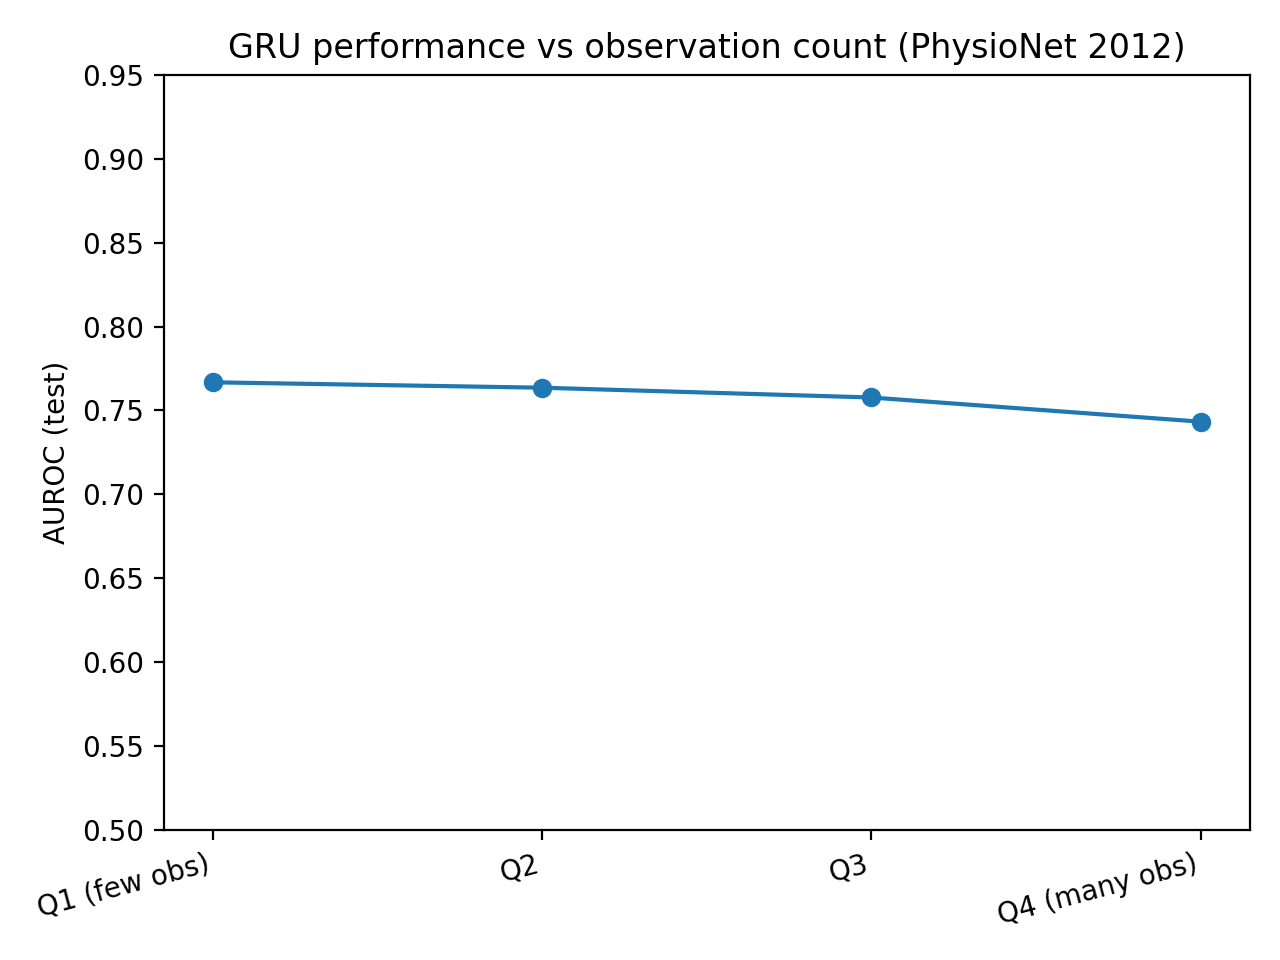
\includegraphics[width=0.95\linewidth]{../results/figures/physio_auroc_by_obs_quartile.png}
\caption{GRU test AUROC stratified by observation-count quartile (fewer observations $\rightarrow$ harder cases).}
\label{fig:physio_obs}
\end{figure}
\section{Limitations and future work}
This study is intentionally minimal. Key limitations include:
\begin{itemize}
  \item \textbf{Toy dataset:} a damped oscillator is smooth and low-dimensional; benefits may shrink on noisy, high-dimensional, or discontinuous dynamics.
  \item \textbf{Single baseline family:} the ResNet baseline could be strengthened with explicit time-delta conditioning, interpolation layers, or latent state-space models.
  \item \textbf{Limited sweep:} we do not yet sweep hidden size, depth, regularization, or training budget; results could depend on capacity matching.
  \item \textbf{Compute/solver settings:} tighter solver tolerances or alternative adjoint/solver strategies may matter in larger settings even if not here.
\end{itemize}

Future work: add time-aware discrete baselines (e.g., $\Delta t$-conditioned ResNet, GRU-D), sweep model size, and test on a harder irregularly sampled benchmark.

\vspace{0.5em}
\noindent\textbf{Code and artifacts:} \href{\GithubURL}{\GithubURL} (configs, training logs, summary table, and figures).

\end{document}

